\documentclass[review,12pt]{elsarticle}

\usepackage{amsmath}
\usepackage{graphicx}
\usepackage{booktabs}
\usepackage[colorlinks=true,allcolors=blue]{hyperref}
\graphicspath{{../figures/v1/}}
% generated by scripts/reproduce_paper.py; never edit by hand
\newcommand{\vEOneMsys}{140.99}
\newcommand{\vEOneVsys}{285.59}
\newcommand{\vEOneTwall}{13.59}
\newcommand{\vEtwoGC}{0.0478}
\newcommand{\vEtwoVC}{0.0222}
\newcommand{\vEtwoGCdev}{41}
\newcommand{\vEtwoVCdev}{5.8}
\newcommand{\vHthreeM}{99.6}
\newcommand{\vHthreeV}{184.7}
\newcommand{\vHthreeMdev}{-0.2}
\newcommand{\vHthreeVdev}{-10.6}
\newcommand{\vNmaxLoA}{37}
\newcommand{\vNmaxHiA}{142}
\newcommand{\vLpLoA}{7.79}
\newcommand{\vLpHiA}{12}
\newcommand{\vNmaxLoM}{61.2}
\newcommand{\vNmaxHiM}{62.6}
\newcommand{\vLpLoM}{9.12}
\newcommand{\vLpHiM}{9.18}
\newcommand{\vObjDof}{3.33}
\newcommand{\vGCpropLo}{0.0435}
\newcommand{\vGCpropHi}{0.0457}
\newcommand{\vGCpropPct}{2.4}
\newcommand{\vESSmin}{16247}
\newcommand{\vRhatMax}{1.0031}
\newcommand{\vObjMtwo}{379.7}
\newcommand{\vObjFreeM}{313.6}
\newcommand{\vFreeM}{2.65}
\newcommand{\vObjToth}{2880.8}
\newcommand{\vGCmean}{0.0440}
\newcommand{\vGCsd}{0.0035}
\newcommand{\vShOne}{hx\_vol\_fraction}
\newcommand{\vShOneShare}{0.30}
\newcommand{\vShTwo}{mli\_k\_eff\_factor}
\newcommand{\vShTwoShare}{0.21}
\newcommand{\vShMat}{0.011}
\newcommand{\vUreqVone}{0.120}
\newcommand{\vUreqVzero}{0.065}
\newcommand{\vAxUd}{0.039}
\newcommand{\vAxUdAbs}{0.072}
\newcommand{\vAmbientVint}{659}
\newcommand{\vEtwoGCdevCorr}{37}
\newcommand{\vEtwoGCdevFixed}{51}


\journal{Adsorption}

\begin{document}
\begin{frontmatter}

\title{Single-isotherm non-identifiability of modified Dubinin--Astakhov
parameters and the statement of system-level hydrogen-storage requirements in
observable quantities}

\author{Avin Gupta}
\ead{iamavingupta@gmail.com}
\address{}

\begin{abstract}
System-level targets for onboard hydrogen storage are routinely translated
into required sorbent properties through the modified Dubinin--Astakhov (D--A)
isotherm. We quantify how much of that translation a single published
isotherm can support. Two independent digitization routes, reconciled under a
pre-registered rule with per-point uncertainties, recover eleven
AX-21 excess isotherms (30--298\,K) from the literature; profile likelihoods
under an explicit errors-in-pressure measurement model show that one 77\,K
isotherm of ordinary published quality leaves the D--A parameter vector
practically non-identifiable (95\% region $n_{\max}$
\vNmaxLoA--\vNmaxHiA\,mol\,kg$^{-1}$ under the frozen parameter bounds, and
wider still when they are relaxed; $\log_{10}P_0$ unbounded above within
[\vLpLoA, \vLpHiA]), while seven supercritical isotherms fitted jointly pin
$n_{\max}$ to \vNmaxLoM--\vNmaxHiM\,mol\,kg$^{-1}$ --- a within-model
precision: model-form and fit-set choice move the centre by $\pm13\%$. Propagated through a
component-resolved system model, the loose single-isotherm region changes
predicted usable system capacity by only about $\pm$\vGCpropPct\%: the model
is sloppy, with loose parameters and tight predictions, so a requirement
stated as a limiting uptake at fixed energetic parameters is conditional on a
ridge the data do not resolve. The engineering model itself was calibrated on
one published HSECoE system and evaluated once against externally
pre-registered held-out targets; three of four comparisons passed and the
200-bar gravimetric comparison failed (+\vEtwoGCdev\% against a $\pm$20\%
band), so, per the pre-registered fork rule, no absolute system capacity is
claimed and requirement maps are reported in observable axes---deliverable
excess uptake between stated full and empty states, and packing
density---under two structurally different engineering models. Shapley-effect attribution over the joint
posterior and declared engineering uncertainties shows engineering inputs,
not material-parameter uncertainty, dominate the variance of predicted
capacity. All data, code, analyses and this manuscript's numbers regenerate
from a single open repository.
\end{abstract}

\begin{keyword}
hydrogen storage \sep cryo-adsorption \sep Dubinin--Astakhov \sep
identifiability \sep uncertainty quantification \sep pre-registration
\end{keyword}

\end{frontmatter}

\section{Introduction}

Vehicle-level targets for onboard hydrogen storage are stated for complete
systems on a usable basis~\cite{usdrive2017}, while materials papers report
excess uptake at material level. The Hydrogen Storage Engineering Center of
Excellence (HSECoE) built the reference translation between the two: detailed
and system-level models of cryo-adsorbent
systems~\cite{hardy2012,tamburello2017,purewal2019}, an Adsorbent
Acceptability Envelope that back-calculates material requirements from system
targets~\cite{hardy2018,corgnale2012,pasini2013}, and Argonne's sorbent
property requirements stated
directly in measurable quantities~\cite{ahluwalia2015}. The present work is
not the first inversion of system targets into material requirements; those
programs are its reference point.

This paper asks a narrower statistical question underneath that translation:
when the material is characterized by the modified D--A
model~\cite{richard2009a} fitted to the single-temperature excess isotherms
the literature routinely publishes, which parameter combinations does the
data determine, and what does the answer imply for how requirements should be
stated? Three contributions follow. First, an identifiability analysis ---
profile likelihoods under an explicit measurement-error model with error in
pressure as well as uptake --- of the D--A parameter vector against a
dual-digitized, uncertainty-tagged reconstruction of the classic AX-21
dataset~\cite{benard2001,richard2009a}, quantifying both the single-isotherm
degeneracy and its repair by multi-temperature fitting. Second, the
propagation of parameter uncertainty through an openly implemented,
component-resolved system model whose calibration and held-out validation
were frozen by an external, time-stamped pre-registration before the model
code existed~\cite{prereg}, with the held-out outcome --- including one
pre-registered failure --- reported and binding on the claims. Third,
requirement maps stated in observable axes, following the practice of the
HSECoE envelope and the Argonne targets, drawn under two independent
engineering models so the model-dependence of the boundary is an exhibit
rather than a hidden assumption.

The $\alpha$--$\beta$ degeneracy at a single temperature is structural
($\varepsilon=\alpha+\beta T$) and was implicitly recognized by the original
authors, who fitted all temperatures jointly and published alternative
parameter sets of comparable quality~\cite{richard2009a}; the
adsorbed-volume ambiguity of supercritical excess data is likewise
long-standing~\cite{myers2014}. What this paper adds is the quantification:
how loose the single-isotherm region actually is under an honest error
model, how tightly it nonetheless constrains system-level predictions
(``sloppiness'' in the sense of Gutenkunst et
al.~\cite{gutenkunst2007}), and what statement of requirements survives
that structure.

\section{Data}

\subsection{Dual digitization and reconciliation}

No numeric tables of the multi-temperature AX-21 isotherms are published:
the measurements of B\'enard and Chahine~\cite{benard2001} appear as figures
there and in Richard et al.~\cite{richard2009a} (Fig.~1a). Figure~1a was
digitized at 600\,dpi by two independent routes --- a visual marker-by-marker
reading and a scripted template-matching pipeline, executed in isolation
from each other --- and reconciled under a rule frozen in the
pre-registration before either output was read: nearest-pressure matching,
coordinate-wise means within tolerance, one documented re-inspection of
disagreements, exclusion (with counts) of markers neither route resolves.
The result is 172 points on eleven isotherms (Fig.~\ref{fig:fit}) with
per-point uncertainties floored at the axis resolution (0.0049\,MPa and 0.062\,mol\,kg$^{-1}$ per
pixel); 21 of 22 systematic disagreements traced to a marker-center
convention difference on the two triangle-marker isotherms and were settled
by direct measurement of isolated glyphs. Two Henry-region points lie within
one pixel of the pressure axis and are recorded at the half-pixel bound with
matching uncertainty. The 30\,K isotherm lies below the validity floor of
the gas-phase equation of state (33.2\,K) and enters no fit. The SWCNT
isotherms of Panella et al.~\cite{panella2005} (Fig.~2b) were digitized
under the same protocol, including the published error bars.

\begin{figure}[t]
\centering
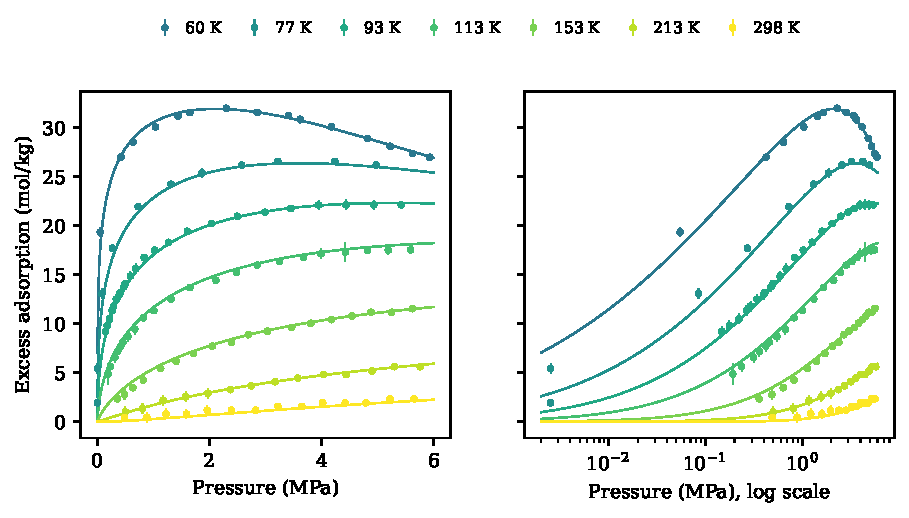
\includegraphics[width=\linewidth]{F2_multiT_fit}
\caption{The seven supercritical (60--298\,K) isotherms of the reconciled
dual-digitized AX-21 dataset (points, with error-model uncertainties) and
the joint modified D--A fit (curves). The dataset's 30--45\,K subcritical
isotherms enter no primary fit: 35--45\,K are excluded by the frozen
analysis plan, and 30\,K lies below the equation-of-state validity floor.}
\label{fig:fit}
\end{figure}

\subsection{Measurement-error model}

Every fit minimizes
$\sum_i (n_{\mathrm{model},i}-n_i)^2/\sigma_{\mathrm{eff},i}^2$ with
$\sigma_{\mathrm{eff},i}^2=\sigma_{n,i}^2+(\partial n/\partial
P|_i)^2\sigma_{P,i}^2$, the first-order errors-in-abscissa propagation, with
the derivative evaluated analytically on the model. On the steep Henry
branch this discounts near-axis points in proportion to what the pixel grid
resolves, which removes by construction the known failure mode in which
sub-pixel low-pressure points dominate a fitted covariance. Residuals remain
overdispersed relative to digitization uncertainty alone
(objective/dof $=\vObjDof$), which measures residual model-form error
(Section~\ref{sec:modelform}); intervals are therefore reported at both the
nominal $\Delta=3.84$ threshold and the variance-inflated threshold, and no
conclusion relies on the narrower of the two.

\section{Models}

\subsection{Isotherm, bookkeeping and gas phase}

Absolute adsorption follows the modified D--A form
$n_{\mathrm{abs}}=n_{\max}\exp[-(RT/\varepsilon)^m\ln^m(P_0/P)]$ with
$\varepsilon=\alpha+\beta T$ and $m=2$ unless stated; excess is
$n_{\mathrm{ex}}=n_{\mathrm{abs}}-\rho_g(P,T)\,v_a$~\cite{richard2009a}.
Gas densities use the Leachman normal-hydrogen reference equation of
state~\cite{leachman2009} via CoolProp~\cite{bell2014}; the wrapper
reproduces the NIST tables to $5\times10^{-5}$ relative (a plumbing check,
not physics validation). Tank inventory uses absolute loading plus void gas
with the void excluding skeleton and adsorbed volume; usable capacity is the
full-to-empty swing, and system capacities are usable-basis with the full
inventory carried in the system mass.

\subsection{Component-resolved engineering model and pre-registered gates}
\label{sec:gates}

The engineering model resolves the system into composite or aluminium
vessel (netting analysis for composite: helical plies carry the axial load,
total cylinder thickness $1.5\,P r/\sigma$ exactly; hoop-governed wall for
aluminium), fixed-thickness liner, multilayer insulation sized to a
heat-leak budget at 60\,$^\circ$C ambient or fixed at the design value,
outer shell, internal heat-exchanger structure, supports, and a
component-class balance of plant carrying mass and volume, with the design
pressure set by the dormancy vent rule $P_\mathrm{design}=1.25\,P_\mathrm{full}$
\cite{ahluwalia2009,tamburello2017,purewal2019}. Three bounded scalar
factors are the model's only fitted values.

Calibration and validation were frozen by an external, DOI-stamped
pre-registration before any model code existed~\cite{prereg}: calibrate on
the published HexCell system specification~\cite{tamburello2017} and
evaluate once against held-out HSECoE AX-21 anchors with fixed targets,
tolerances, and a fork rule. We state the deposit's evidential force
precisely: the whole arc from deposit to adjudication spans about a hundred
minutes of one day, with the model necessarily developed alongside, so the
deposit certifies that the targets, tolerances and fork rule were fixed and
externally timestamped before the outcomes were known --- the adjudicated
failure below, and the enforcement of the fork rule, are the behaviour
consistent with that discipline --- and it supports no stronger reading.
The repository records the execution deviations from the frozen text, each
dated and quantified. Calibration closed to $\vEOneMsys$\,kg against
140.99\,kg and $\vEOneVsys$\,L against 287.70\,L (wall \vEOneTwall\,mm vs
14.00\,mm). The held-out gate (Table~\ref{tab:gates}; note that the 200-bar
cases evaluate the AX-21 parameter set at 20\,MPa, $3.3\times$ beyond its
0--6\,MPa fit range --- the anchors themselves model 200\,bar, but the
extrapolation is one more uncertainty those two comparisons carry): the 60\,bar/40\,K aluminium system matched to
$\vHthreeMdev$\% in mass and $\vHthreeVdev$\% in volume (both PASS at
$\pm25\%$), the 200-bar composite system's volumetric capacity passed
(+\vEtwoVCdev\% at $\pm20\%$), and its gravimetric capacity failed
(+\vEtwoGCdev\% against $\pm20\%$). \textbf{The gate therefore failed}, and
the pre-registered fork rule governs this paper: no absolute system capacity
is claimed; relative statements beyond monotone orderings appear only with
the two-model robustness exhibit of Section~\ref{sec:observables}. We note,
as disclosed context rather than mitigation, that the anchor family itself
spans 21\% across HSECoE report years for the nominal same configuration and
does not state its capacity basis; and that the failure is mass-sided and
pressure-dependent, consistent with build features (boss reinforcement,
doilies, protective layers) that pure netting sizing omits.

A post-adjudication audit additionally found one model input mis-attributed:
the balance-of-plant interpolation's 16\,kg anchor was placed at 100\,bar,
while its source states it as a fixed assumption of a 150\,atm-storage
analysis. The gate record stands as adjudicated; re-anchoring at the
source's own pressures moves the failed comparison to $+\vEtwoGCdevCorr\%$
(or $+\vEtwoGCdevFixed\%$ treating the anchor as pressure-independent, as
its source does) and flips no verdict, so the fork rule is robust to the
correction (sensitivity committed in the repository).

\begin{table}[t]
\centering
\caption{Pre-registered calibration (E1) and held-out validation (E2)
outcomes~\cite{prereg}. Targets are the published HSECoE values; tolerances
and the all-four pass rule were frozen and DOI-stamped before any model code
existed. E1 is in-sample by construction; E2 is the evidence.}
\label{tab:gates}
\begin{tabular}{llll}
\toprule
 & Quantity & Deviation (tolerance) & Verdict \\
\midrule
E1 & system mass & \vEOneMsys\,kg vs 140.99\,kg & calibrated \\
E1 & system volume & \vEOneVsys\,L vs 287.70\,L & calibrated \\
\midrule
E2 & 200\,bar/80\,K gravimetric & $+\vEtwoGCdev\%$ ($\pm20\%$) & \textbf{FAIL} \\
E2 & 200\,bar/80\,K volumetric & $+\vEtwoVCdev\%$ ($\pm20\%$) & pass \\
E2 & 60\,bar/40\,K system mass & $\vHthreeMdev\%$ ($\pm25\%$) & pass \\
E2 & 60\,bar/40\,K system volume & $\vHthreeVdev\%$ ($\pm25\%$) & pass \\
\midrule
\multicolumn{4}{l}{Gate E2 (pass iff all four): \textbf{FAIL} --- the
pre-registered fork rule governs all claims.} \\
\midrule
 & \multicolumn{3}{l}{Context: the same 200-bar prediction against the
   anchor family's} \\
 & \multicolumn{3}{l}{other report years (not gate criteria): FY2011
   $+22.6\%$; ST044-2012} \\
 & \multicolumn{3}{l}{$+30.4\%$; ST044-2013 $+53.2\%$ --- the family itself
   spans 21\%.} \\
\bottomrule
\end{tabular}
\end{table}

\section{Identifiability}

Profile likelihoods~\cite{raue2009} were computed for every parameter,
re-optimizing the others at each fixed value, with interval endpoints located
by bisection;
bounds are physical ($P_0$ above the fitted pressure range, with the
bound-relaxation sensitivity reported in the repository). From the single
77\,K isotherm (Fig.~\ref{fig:profiles}), the 95\% region spans $n_{\max}$ from \vNmaxLoA{} to
\vNmaxHiA\,mol\,kg$^{-1}$ and $\log_{10}(P_0/\mathrm{Pa})$ from \vLpLoA{} to
the upper bound \vLpHiA{}; $\beta$ is undetermined at one temperature by
construction, and $\alpha$ is identified only through
$\varepsilon(77)$. The 77\,K interval endpoints are conditional on the
frozen $\log_{10}(P_0/\mathrm{Pa})\le12$ bound: raising it to 14 widens
$n_{\max}$ to 38--263 (committed sensitivity), which strengthens the
non-identifiability conclusion. From the seven supercritical isotherms
fitted jointly, the same intervals collapse to
\vNmaxLoM--\vNmaxHiM\,mol\,kg$^{-1}$ ($\pm$1.2\%; $\beta$ $\pm$2.0\%, $v_a$
$\pm$2.4\%) and \vLpLoM--\vLpHiM{}: the degeneracy is a property of
single-temperature reporting practice, not of the model class, and
multi-temperature fitting restores identifiability by nearly two orders of
magnitude in interval width. That precision is within-model: freeing the
D--A exponent moves $n_{\max}$ to 54.4, adding the 35--45\,K subcritical
isotherms moves it to 69.2, and the source's own 30--293\,K global fit is
71.6~\cite{richard2009a} --- a $\pm13\%$ structural spread that any use of
the within-model interval must carry with it (the overdispersion-inflated
intervals, roughly twice the frozen ones, are the decisive in-model
statement given Section~\ref{sec:modelform}). The Fisher-information spectrum in log-parameter coordinates spans
several decades at the optimum --- the signature of a sloppy
model~\cite{gutenkunst2007}.

An MCMC posterior over the same objective (uniform priors on the frozen
bounds; effective sample size $\ge\vESSmin$ per parameter, split-chain
$\hat R \le \vRhatMax$) matches the profile intervals and supplies the joint
input distribution for Section~\ref{sec:uq}.

\begin{figure}[t]
\centering
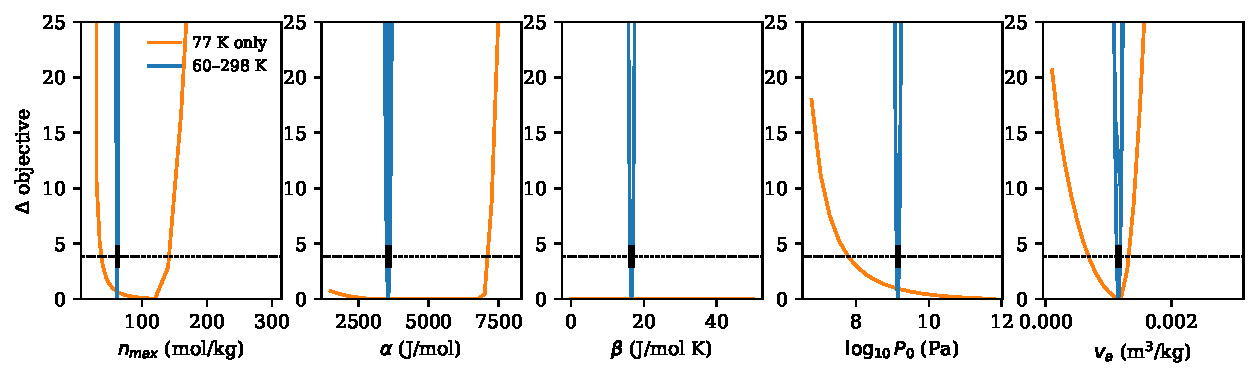
\includegraphics[width=\linewidth]{F3_profiles}
\caption{Profile likelihoods for the modified D--A parameters from the
single 77\,K isotherm (broad curves) and from the seven supercritical
isotherms fitted jointly (narrow curves), with the 95\% threshold. At one
temperature, $n_{\max}$ and $\log_{10}P_0$ are practically non-identifiable
and $\beta$ is structurally undetermined; the multi-temperature fit
restores identifiability.}
\label{fig:profiles}
\end{figure}


\subsection{Model form}
\label{sec:modelform}

Fitting the exponent freely prefers $m=\vFreeM$ (objective \vObjFreeM{}
against \vObjMtwo{} at $m=2$), while a T\'oth form fits far worse
(\vObjToth); the $m=2$ restriction is the dominant residual
misspecification, is visible as the overdispersion above, and is carried in
the reported intervals rather than ignored.

\section{Loose parameters, tight predictions}

Propagating the 77\,K profile ridge (a 3.0-fold range in $n_{\max}$ on the
propagated grid; the full 95\% interval is 3.8-fold) through the frozen
engineering model at the baseline envelope (100\,bar/80\,K to
5\,bar/160\,K) changes predicted usable gravimetric capacity only between
\vGCpropLo{} and \vGCpropHi{} ($\pm$\vGCpropPct\%; Fig.~\ref{fig:ridge});
evaluated at the exact interval endpoints it stays within about 4\% of the
optimum.

\begin{figure}[t]
\centering
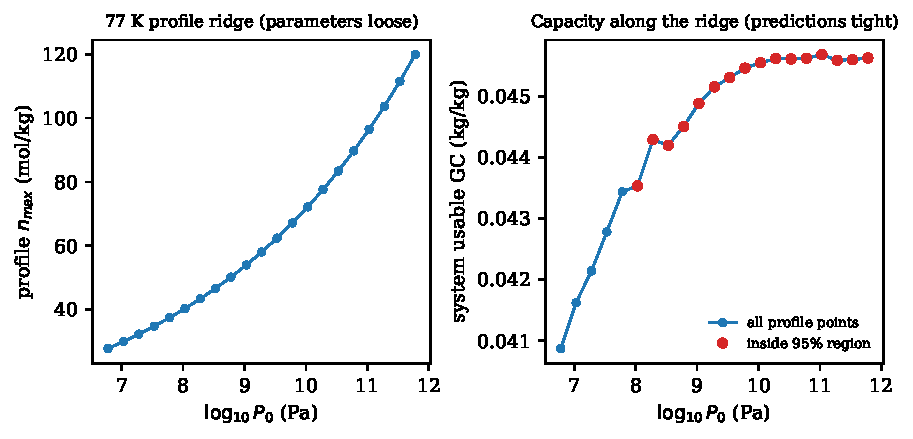
\includegraphics[width=\linewidth]{F6_sloppiness}
\caption{Loose parameters, tight predictions. Left: the 77\,K profile ridge
--- equally admissible $(n_{\max},\log_{10}P_0)$ pairs spanning a 3.8-fold
range in $n_{\max}$. Right: usable system gravimetric capacity along the
same ridge under the frozen engineering model; points inside the 95\%
profile region are highlighted. The data leave the parameters loose while
pinning the prediction.}
\label{fig:ridge}
\end{figure}
The practical consequence is the paper's central point: a requirement stated
as ``$n_{\max}=X$ at fixed $\alpha,\beta,P_0$'' is conditional on an
arbitrary point along a ridge that single-isotherm data do not resolve ---
the same material, described by equally admissible parameter vectors, can
``have'' an $n_{\max}$ anywhere across a wide interval with essentially
unchanged system behaviour. Requirements must therefore be stated in
quantities the data determine.

\section{Uncertainty attribution}
\label{sec:uq}

With material parameters drawn from the joint posterior and fifteen
declared engineering and envelope inputs drawn from documented
distributions, the usable-capacity distribution at the baseline envelope has
mean \vGCmean{} and standard deviation \vGCsd{} (N=20{,}000; split-half
quantile agreement recorded). Shapley effects --- the variance attribution
appropriate to dependent inputs~\cite{song2016,owen2014}
(Fig.~\ref{fig:shapley}) --- rank the
internal heat-exchanger structure (\vShOneShare{} of variance), insulation
conductivity (\vShTwoShare) and heat-leak budget ahead of everything else,
with the correlated material block contributing only \vShMat{} of the
variance. Material-parameter uncertainty, once its correlations are
respected, is a minor contributor; the engineering description dominates.
Design-leverage elasticities are reported separately from variance shares,
since a large variance share reflects declared ignorance, not improvement
potential.

\begin{figure}[t]
\centering
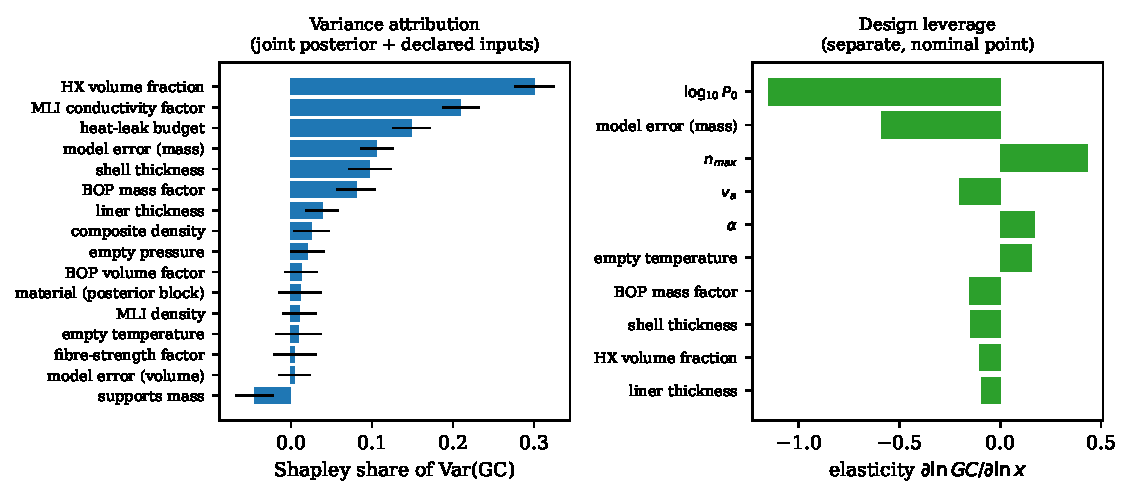
\includegraphics[width=\linewidth]{F7_shapley_elasticity}
\caption{Left: Shapley effects (variance shares) for usable gravimetric
capacity over the joint material posterior and the fifteen declared
engineering inputs; the correlated material block is one player. Shares
within two standard errors of zero (error bars) are indistinguishable from
zero. Right: design-leverage elasticities of the same output, which answer
a different question and are deliberately not merged with the variance
shares.}
\label{fig:shapley}
\end{figure}

\section{Requirements in observables}
\label{sec:observables}

The requirement map uses deliverable \emph{excess} uptake between the
stated full and empty states, together with packing density, as axes ---
quantities measurable without inverting an isotherm model, as in the HSECoE
envelope~\cite{hardy2018} and the Argonne Level-1
targets~\cite{ahluwalia2015} (120\,g\,kg$^{-1}$ excess at 100\,bar/155\,K
and 420\,kg\,m$^{-3}$ bulk density for the 40\,g\,L$^{-1}$ system target).
The basis matters: on the excess basis the adsorbed-phase volume $v_a$
drops out of the bed-level inventory algebraically (the gas swing rides on
the total void $1-\rho/\rho_{\mathrm{skel}}$), so the axis needs only the
measured excess swing, the packing density, a skeletal density and the
equation of state; an absolute-adsorption axis would re-import the fitted,
poorly identified $v_a$, which at this envelope shifts a material's
coordinate by $v_a\,\Delta\rho_g = 0.034$\,kg\,kg$^{-1}$ --- half of
AX-21's own value. The skeletal-density and residual-uptake terms are
varied as labelled sensitivities in the repository (over
1800--2300\,kg\,m$^{-3}$ the required uptake at 500\,kg\,m$^{-3}$ packing
moves by 0.004\,kg\,kg$^{-1}$; the residual-uptake term does not move the
boundary there, which is volumetric-limited).
No probability band is drawn on these axes: they are observables, not
sampled parameters. Under the component-resolved model (Fig.~\ref{fig:map}), meeting the
DOE-2025 pair at 500\,kg\,m$^{-3}$ packing requires a deliverable excess
uptake of about \vUreqVone\,kg\,kg$^{-1}$; under the superseded lumped
model the same contour sits at \vUreqVzero{} --- the between-model shift is
of the same order as the held-out failure and is displayed as the honest
statement of how model-dependent such boundaries are, with the caveat that
the two models share several source anchors (insulation properties, the
balance-of-plant anchor, the fibre class), so the displayed shift is a
lower bound on engineering-model dependence. AX-21's deliverable excess
uptake at this envelope is \vAxUd\,kg\,kg$^{-1}$ (posterior median;
\vAxUdAbs{} on the absolute basis), far from feasibility at any packing
density, consistent with the HSECoE conclusion that
roughly 20\,wt\% material-level capacity underlies the 5.5\,wt\% system
target~\cite{hardy2018}. The ambient (298\,K) configuration appears only as
a supplementary contrast: its tank sizes to \vAmbientVint\,L for 5.6\,kg
usable.

\begin{figure}[t]
\centering
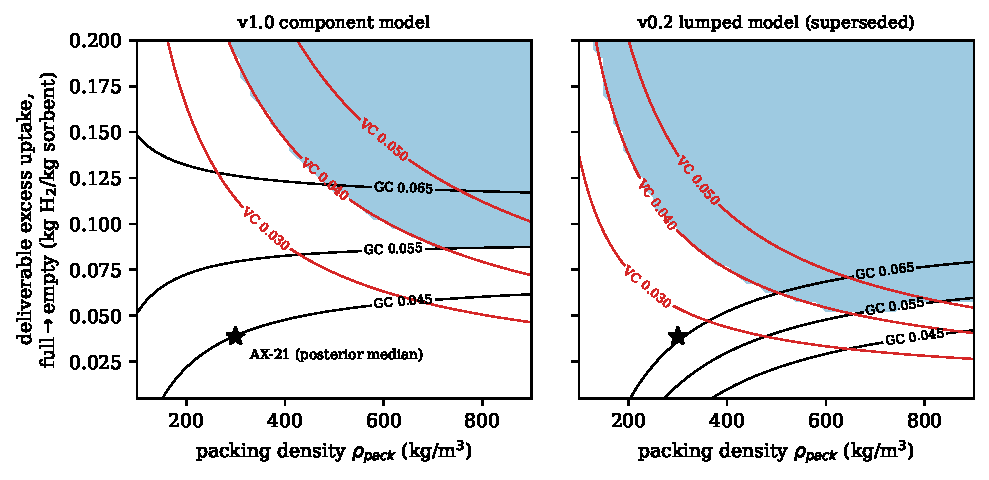
\includegraphics[width=\linewidth]{F5_observable_map}
\caption{System feasibility stated in observable axes: deliverable
\emph{excess} uptake between the stated full (100\,bar/80\,K) and empty
(5\,bar/160\,K) states versus packing density, with the DOE-2025
requirement region under the component-resolved model (left) and the
superseded lumped model (right). The between-model shift is a lower bound
on how model-dependent such boundaries are (the models share several source
anchors); AX-21's posterior-median deliverable excess uptake is marked.}
\label{fig:map}
\end{figure}

\section{Limitations}

The engineering gate failed and every absolute capacity here is
conditional; the data are figure-digitized with stated resolution; the
$m=2$ misspecification dominates residuals; several engineering input
distributions rest on single published data, and the Shapley analysis says
precisely those dominate the output variance; the only traceable 77\,K
high-pressure CNT isotherm reconciles to five points, below the
pre-registered floor, so no CNT system claim is made (the repository carries
the documented example, consistent with
\cite{tibbetts2001,panella2005,zhou2004}). The repository's
\texttt{known\_limitations} document is the complete register.

\section{Conclusions}

A single published isotherm does not determine the modified D--A parameter
vector, but it does determine system-level predictions to a few per cent;
multi-temperature data restore parameter identifiability almost completely.
Requirements derived from system targets should therefore be stated in
deliverable uptake and packing density --- observable, model-robust axes ---
with the engineering model's own validation status attached, which in this
work is an externally pre-registered calibration that passed and a held-out
gate that failed and narrowed the claims. The companion database
(HyCAN-DB~\cite{hycandb}) and this model are one program: curating
multi-temperature, provenance-tiered measurements is what makes the
translation from materials to systems identifiable at all.

\section*{Methods: computational and AI involvement}

All analyses are deterministic-seeded and regenerate from the repository
(\texttt{scripts/}); this manuscript's numbers are compiled from a
machine-generated macro file, and a test fails if manuscript and
regeneration disagree. Anthropic Claude (claude.ai, 2026 releases) was used
throughout the research process under a version-controlled execution manual
and an externally deposited pre-registration~\cite{prereg}: it implemented
the models and analyses, performed the dual figure digitizations as two
isolated agent instances and their frozen-rule reconciliation, retrieved and
DOI-verified the literature, drafted documentation and this manuscript, and
executed the pre-registered gates. The author verified every load-bearing
input value against its primary source, froze the pre-registered decisions
including the held-out tolerances and fork rule, holds sole responsibility
for all content, and reviewed and edited all AI-produced text and analysis.
The repository's \texttt{docs/ai\_usage\_log.md} is the contemporaneous
record. AI tools were not used to create or alter any primary data; the
digitized datasets carry both routes' raw readings.

\section*{Declaration of generative AI and AI-assisted technologies in the manuscript preparation process}

During the preparation of this work the author used Anthropic Claude in
order to draft and revise the manuscript text and generate the figures from
the committed analysis records. After using this tool, the author reviewed
and edited the content as needed and takes full responsibility for the
content of the published article.

\section*{Data availability}

All data, code, figures and analysis records are openly available at
\url{https://github.com/AvinGupta-ship-it/h2star} (archived at Zenodo,
concept DOI 10.5281/zenodo.23257816; the pre-registration is
10.5281/zenodo.23931242).

\bibliographystyle{elsarticle-num}
\begin{thebibliography}{30}

\bibitem{usdrive2017} U.S. DRIVE Partnership, Target Explanation Document:
Onboard Hydrogen Storage for Light-Duty Fuel Cell Vehicles, updated May
2017.

\bibitem{hardy2012} B. Hardy, C. Corgnale, D. Tamburello, S. Garrison, D.
Anton, et al., Modeling of adsorbent based hydrogen storage systems, Int. J.
Hydrogen Energy 37 (2012) 5691--5705. doi:10.1016/j.ijhydene.2011.12.125.

\bibitem{tamburello2017} D. Tamburello, B. Hardy, C. Corgnale, M. Sulic, D.
Anton, Cryo-adsorbent hydrogen storage systems for fuel cell vehicles,
Proc.\ ASME FEDSM2017, FEDSM2017-69411. doi:10.1115/FEDSM2017-69411.

\bibitem{purewal2019} J. Purewal, M. Veenstra, D. Tamburello, A. Ahmed, A.
Matzger, A. Wong-Foy, S. Seth, Y. Liu, D. Siegel, Estimation of
system-level hydrogen storage for metal-organic frameworks with high
volumetric storage density, Int. J. Hydrogen Energy 44 (2019) 15135--15145.
doi:10.1016/j.ijhydene.2019.04.082.

\bibitem{hardy2018} B. Hardy, D. Tamburello, C. Corgnale, Hydrogen storage
adsorbent systems acceptability envelope, Int. J. Hydrogen Energy 43 (2018)
19528--19539. doi:10.1016/j.ijhydene.2018.08.140.

\bibitem{ahluwalia2015} R.K. Ahluwalia, J.K. Peng, T.Q. Hua, Sorbent
material property requirements for on-board hydrogen storage for automotive
fuel cell systems, Int. J. Hydrogen Energy 40 (2015) 6373--6390.
doi:10.1016/j.ijhydene.2015.03.025.

\bibitem{richard2009a} M.-A. Richard, P. B\'enard, R. Chahine, Gas
adsorption process in activated carbon over a wide temperature range above
the critical point. Part 1: modified Dubinin-Astakhov model, Adsorption 15
(2009) 43--51. doi:10.1007/s10450-009-9149-x.

\bibitem{benard2001} P. B\'enard, R. Chahine, Determination of the
adsorption isotherms of hydrogen on activated carbons above the critical
temperature of the adsorbate over wide temperature and pressure ranges,
Langmuir 17 (2001) 1950--1955. doi:10.1021/la001381x.

\bibitem{panella2005} B. Panella, M. Hirscher, S. Roth, Hydrogen adsorption
in different carbon nanostructures, Carbon 43 (2005) 2209--2214.
doi:10.1016/j.carbon.2005.03.037.

\bibitem{myers2014} A.L. Myers, P.A. Monson, Physical adsorption of gases:
the case for absolute adsorption as the basis for thermodynamic analysis,
Adsorption 20 (2014) 591--622. doi:10.1007/s10450-014-9604-1.

\bibitem{gutenkunst2007} R.N. Gutenkunst, J.J. Waterfall, F.P. Casey, K.S.
Brown, C.R. Myers, J.P. Sethna, Universally sloppy parameter sensitivities
in systems biology models, PLoS Comput. Biol. 3 (2007) e189.
doi:10.1371/journal.pcbi.0030189.

\bibitem{raue2009} A. Raue, C. Kreutz, T. Maiwald, J. Bachmann, M. Schilling,
U. Klingm\"uller, J. Timmer, Structural and practical identifiability
analysis of partially observed dynamical models by exploiting the profile
likelihood, Bioinformatics 25 (2009) 1923--1929.
doi:10.1093/bioinformatics/btp358.

\bibitem{leachman2009} J.W. Leachman, R.T. Jacobsen, S.G. Penoncello, E.W.
Lemmon, Fundamental equations of state for parahydrogen, normal hydrogen,
and orthohydrogen, J. Phys. Chem. Ref. Data 38 (2009) 721--748.
doi:10.1063/1.3160306.

\bibitem{bell2014} I.H. Bell, J. Wronski, S. Quoilin, V. Lemort, Pure and
pseudo-pure fluid thermophysical property evaluation and the open-source
thermophysical property library CoolProp, Ind. Eng. Chem. Res. 53 (2014)
2498--2508. doi:10.1021/ie4033999.

\bibitem{ahluwalia2009} R.K. Ahluwalia, J.K. Peng, Automotive hydrogen
storage system using cryo-adsorption on activated carbon, Int. J. Hydrogen
Energy 34 (2009) 5476--5487. doi:10.1016/j.ijhydene.2009.05.023.

\bibitem{song2016} E. Song, B.L. Nelson, J. Staum, Shapley effects for
global sensitivity analysis: theory and computation, SIAM/ASA J. Uncertain.
Quantif. 4 (2016) 1060--1083. doi:10.1137/15M1048070.

\bibitem{owen2014} A.B. Owen, Sobol' indices and Shapley value, SIAM/ASA J.
Uncertain. Quantif. 2 (2014) 245--251. doi:10.1137/130936233.

\bibitem{tibbetts2001} G.G. Tibbetts, G.P. Meisner, C.H. Olk, Hydrogen
storage capacity of carbon nanotubes, filaments, and vapor-grown fibers,
Carbon 39 (2001) 2291--2301. doi:10.1016/S0008-6223(01)00051-3.

\bibitem{zhou2004} L. Zhou, Y. Zhou, Y. Sun, A comparative study of
hydrogen adsorption on superactivated carbon versus carbon nanotubes, Int.
J. Hydrogen Energy 29 (2004) 475--479. doi:10.1016/S0360-3199(03)00092-2.

\bibitem{corgnale2012} C. Corgnale, B. Hardy, D. Tamburello, S. Garrison,
D. Anton, Acceptability envelope for metal hydride-based hydrogen storage
systems, Int. J. Hydrogen Energy 37 (2012) 2812--2824.
doi:10.1016/j.ijhydene.2011.07.037.

\bibitem{pasini2013} J.M. Pasini, C. Corgnale, B.A. van Hassel, T. Motyka,
S. Kumar, K. Simmons, Metal hydride material requirements for automotive
hydrogen storage systems, Int. J. Hydrogen Energy 38 (2013) 9755--9765.
doi:10.1016/j.ijhydene.2012.08.112.

\bibitem{hycandb} A. Gupta, HyCAN-DB: a FAIR database of hydrogen sorption
measurements in carbon nanomaterials, Zenodo (2026).
doi:10.5281/zenodo.23231985.

\bibitem{prereg} A. Gupta, H2STAR v1.0: pre-registration of validation
gates, tolerances, calibration/validation split, and analysis plan, Zenodo
(2026). doi:10.5281/zenodo.23931242.

\end{thebibliography}
\end{document}
